\documentclass[a4paper, 14pt]{extarticle}

% Поля
%--------------------------------------
\usepackage{geometry}
\geometry{a4paper,tmargin=2cm,bmargin=2cm,lmargin=3cm,rmargin=1cm}
%--------------------------------------


%Russian-specific packages
%--------------------------------------
\usepackage[T2A]{fontenc}
\usepackage[utf8]{inputenc} 
\usepackage[english, main=russian]{babel}
%--------------------------------------

\usepackage{textcomp}

% Красная строка
%--------------------------------------
\usepackage{indentfirst}               
%--------------------------------------             


%Graphics
%--------------------------------------
\usepackage{graphicx}
\graphicspath{ {./images/} }
\usepackage{wrapfig}
%--------------------------------------

% Полуторный интервал
%--------------------------------------
\linespread{1.3}                    
%--------------------------------------

%Выравнивание и переносы
%--------------------------------------
% Избавляемся от переполнений
\sloppy
% Запрещаем разрыв страницы после первой строки абзаца
\clubpenalty=10000
% Запрещаем разрыв страницы после последней строки абзаца
\widowpenalty=10000
%--------------------------------------

%Списки
\usepackage{enumitem}

%Подписи
\usepackage{caption} 

%Гиперссылки
\usepackage{hyperref}

\hypersetup {
	unicode=true
}

%Рисунки
%--------------------------------------
\DeclareCaptionLabelSeparator*{emdash}{~--- }
\captionsetup[figure]{labelsep=emdash,font=onehalfspacing,position=bottom}
%--------------------------------------

\usepackage{tempora}

%Листинги
%--------------------------------------
\usepackage{listings}
\lstset{
  basicstyle=\ttfamily\footnotesize, 
  %basicstyle=\footnotesize\AnkaCoder,        % the size of the fonts that are used for the code
  breakatwhitespace=false,         % sets if automatic breaks shoulbd only happen at whitespace
  breaklines=true,                 % sets automatic line breaking
  captionpos=t,                    % sets the caption-position to bottom
  inputencoding=utf8,
  frame=single,                    % adds a frame around the code
  keepspaces=true,                 % keeps spaces in text, useful for keeping indentation of code (possibly needs columns=flexible)
  keywordstyle=\bf,       % keyword style
  numbers=left,                    % where to put the line-numbers; possible values are (none, left, right)
  numbersep=5pt,                   % how far the line-numbers are from the code
  xleftmargin=25pt,
  xrightmargin=25pt,
  showspaces=false,                % show spaces everywhere adding particular underscores; it overrides 'showstringspaces'
  showstringspaces=false,          % underline spaces within strings only
  showtabs=false,                  % show tabs within strings adding particular underscores
  stepnumber=1,                    % the step between two line-numbers. If it's 1, each line will be numbered
  tabsize=2,                       % sets default tabsize to 8 spaces
  title=\lstname                   % show the filename of files included with \lstinputlisting; also try caption instead of title
}
%--------------------------------------

%%% Математические пакеты %%%
%--------------------------------------
\usepackage{amsthm,amsfonts,amsmath,amssymb,amscd}  % Математические дополнения от AMS
\usepackage{mathtools}                              % Добавляет окружение multlined
\usepackage[perpage]{footmisc}
%--------------------------------------

%--------------------------------------
%			НАЧАЛО ДОКУМЕНТА
%--------------------------------------

\begin{document}

%--------------------------------------
%			ТИТУЛЬНЫЙ ЛИСТ
%--------------------------------------
\begin{titlepage}
\thispagestyle{empty}
\newpage


%Шапка титульного листа
%--------------------------------------
\vspace*{-60pt}
\hspace{-65pt}
\begin{minipage}{0.3\textwidth}
\hspace*{-20pt}\centering

\includegraphics[width=\textwidth]{emblem}
\end{minipage}
\begin{minipage}{0.67\textwidth}\small \textbf{
\vspace*{-0.7ex}
\hspace*{-6pt}\centerline{Министерство науки и высшего образования Российской Федерации}
\vspace*{-0.7ex}
\centerline{Федеральное государственное бюджетное образовательное учреждение }
\vspace*{-0.7ex}
\centerline{высшего образования}
\vspace*{-0.7ex}
\centerline{<<Московский государственный технический университет}
\vspace*{-0.7ex}
\centerline{имени Н.Э. Баумана}
\vspace*{-0.7ex}
\centerline{(национальный исследовательский университет)>>}
\vspace*{-0.7ex}
\centerline{(МГТУ им. Н.Э. Баумана)}}
\end{minipage}
%--------------------------------------

%Полосы
%--------------------------------------
\vspace{-25pt}
\hspace{-35pt}\rule{\textwidth}{2.3pt}

\vspace*{-20.3pt}
\hspace{-35pt}\rule{\textwidth}{0.4pt}
%--------------------------------------

\vspace{1.5ex}
\hspace{-35pt} \noindent \small ФАКУЛЬТЕТ\hspace{30pt} <<Информатика, искусственный интеллект и системы управления>>

\vspace*{-16pt}
\hspace{47pt}\rule{0.83\textwidth}{0.4pt}

\vspace{0.5ex}
\hspace{-35pt} \noindent \small КАФЕДРА\hspace{50pt} <<Теоретическая информатика и компьютерные технологии>>

\vspace*{-16pt}
\hspace{30pt}\rule{0.866\textwidth}{0.4pt}
  
\vspace{11em}

\begin{center}
\Large {\bf Лабораторная работа № 0} \\ 
\large {\bf по курсу <<Языки и методы программирования>>} \\
\large <<Приобретение опыта работы с VDS-сервером под управлением ОС Linux>> 
\end{center}\normalsize

\vspace{8em}


\begin{flushright}
  {Студент группы ИУ9-21Б Яннаев А. С. \hspace*{15pt}\\ 
  \vspace{2ex}
  Преподаватель Посевин Д. П.\hspace*{15pt}}
\end{flushright}

\bigskip

\vfill
 

\begin{center}
\textsl{Москва 2025}
\end{center}
\end{titlepage}
%--------------------------------------
%		КОНЕЦ ТИТУЛЬНОГО ЛИСТА
%--------------------------------------

\renewcommand{\ttdefault}{pcr}

\setlength{\tabcolsep}{3pt}
\newpage
\setcounter{page}{2}

\section{Задание}\label{Sect::task}
\begin{enumerate}
\item По инструкции настроить учетную запись на удаленном VDS-сервере.
\item В своей учетной записи настроить окружение для удобного запуска компилятора Java.
\item Запустить любой простейший пример приведенный на лекции 1 или на лабораторной работе 1.
\item Запустить веб-сервер из примера на своем порту. Каждый студент резервирует свой собственный порт. Рекомендуется нумерацию портов использовать по следующему правилу: резервировать номер порта "800n", где n - это порядковый номер студента в Электронном университете, другимим словами, если у студента в Электронном университете порядковй номер 3, то порт веб-сервера данного студента будет 8003.
\item Научиться запускать веб-сервер через утилиту screen.
\item Объединить простейший пример с веб-сервером, т.е. результаты работы программы простейшего прмера выводить через веб-сервер.
\item Запустить работу веб-сервера, выполненного в пункте 6 на своем порту.
\item Как только пункты 1-7 выполнены, выслать строго в телеграм-канал в комментарий к условию данной лабораторной работы: URL-страницы результата работы вашего веб-сервера.
\end{enumerate}
\section{Результаты}\label{Sect::res}

Исходный код программы представлен в ~\ref{lst:code1}.

\begin{figure}[!htb]
\begin{lstlisting}[language={java},caption={Файл HttpServer.java},label={lst:code1}]
import java.io.BufferedReader;
import java.io.IOException;
import java.io.InputStreamReader;
import java.io.PrintWriter;
import java.net.ServerSocket;
import java.net.Socket;
import java.nio.charset.StandardCharsets;

public class HttpServer {

    public static void main(String[] args) {
        try (ServerSocket serverSocket = new ServerSocket(8026)) {
            System.out.println("Server started!");
            
            while (true) {
                Socket socket = serverSocket.accept();
                System.out.println("Client connected!");

                try (BufferedReader input = new BufferedReader(new InputStreamReader(socket.getInputStream(), StandardCharsets.UTF_8));
                     PrintWriter output = new PrintWriter(socket.getOutputStream())) {

                    while (!input.ready()) ;

                    System.out.println();
                    while (input.ready()) {
                        System.out.println(input.readLine());
                    }

                    output.println("HTTP/1.1 200 OK");
                    output.println("Content-Type: text/html; charset=utf-8");
                    output.println();
                    output.println("<p>Hello world!</p>");
		              String[] seasons  = new String[4]; 

                    seasons[0] = "Winter"; 
                    seasons[1] = "Spring"; 
                    seasons[2] = "Summer"; 
                    seasons[3] = "Autumn"; 
                    for (int i = 0; i < 4; i++)
                    {
                        output.println("<p>" + seasons[i] + "</p>");
                    }

                    output.flush();
                    
                    System.out.println("Client disconnected!");
                }
            }
        } catch (IOException ex) {
            ex.printStackTrace();
        }
    }
}

\end{lstlisting}
\end{figure}


Результат запуска представлен на рисунке~\ref{fig:img1}.

\begin{figure}[!htb]
	\centering
	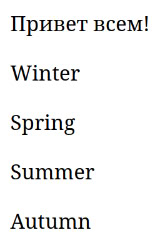
\includegraphics[width=0.4\textwidth]{img1}
\caption{Результат}
\label{fig:img1}
\end{figure}

\end{document}
